\section{CORE in action. Practical Case Study}
\label{sec:corepracticalcasestudy}

The third APRC lab assignment, i.e. OSPF in nine-router topology, was easily set up using the CORE GUI, adding nine routers in a geometrically approximated to the handout's disposition (cf. figure~\ref{fig:kathara-annotated-lab3-topology}), the right links between them, and then extra PC-nodes in a specific ``LAN-prefix'' to test \texttt{iperf3}.

% Figure fig:core-architecture
\begin{figure}
  \centering
  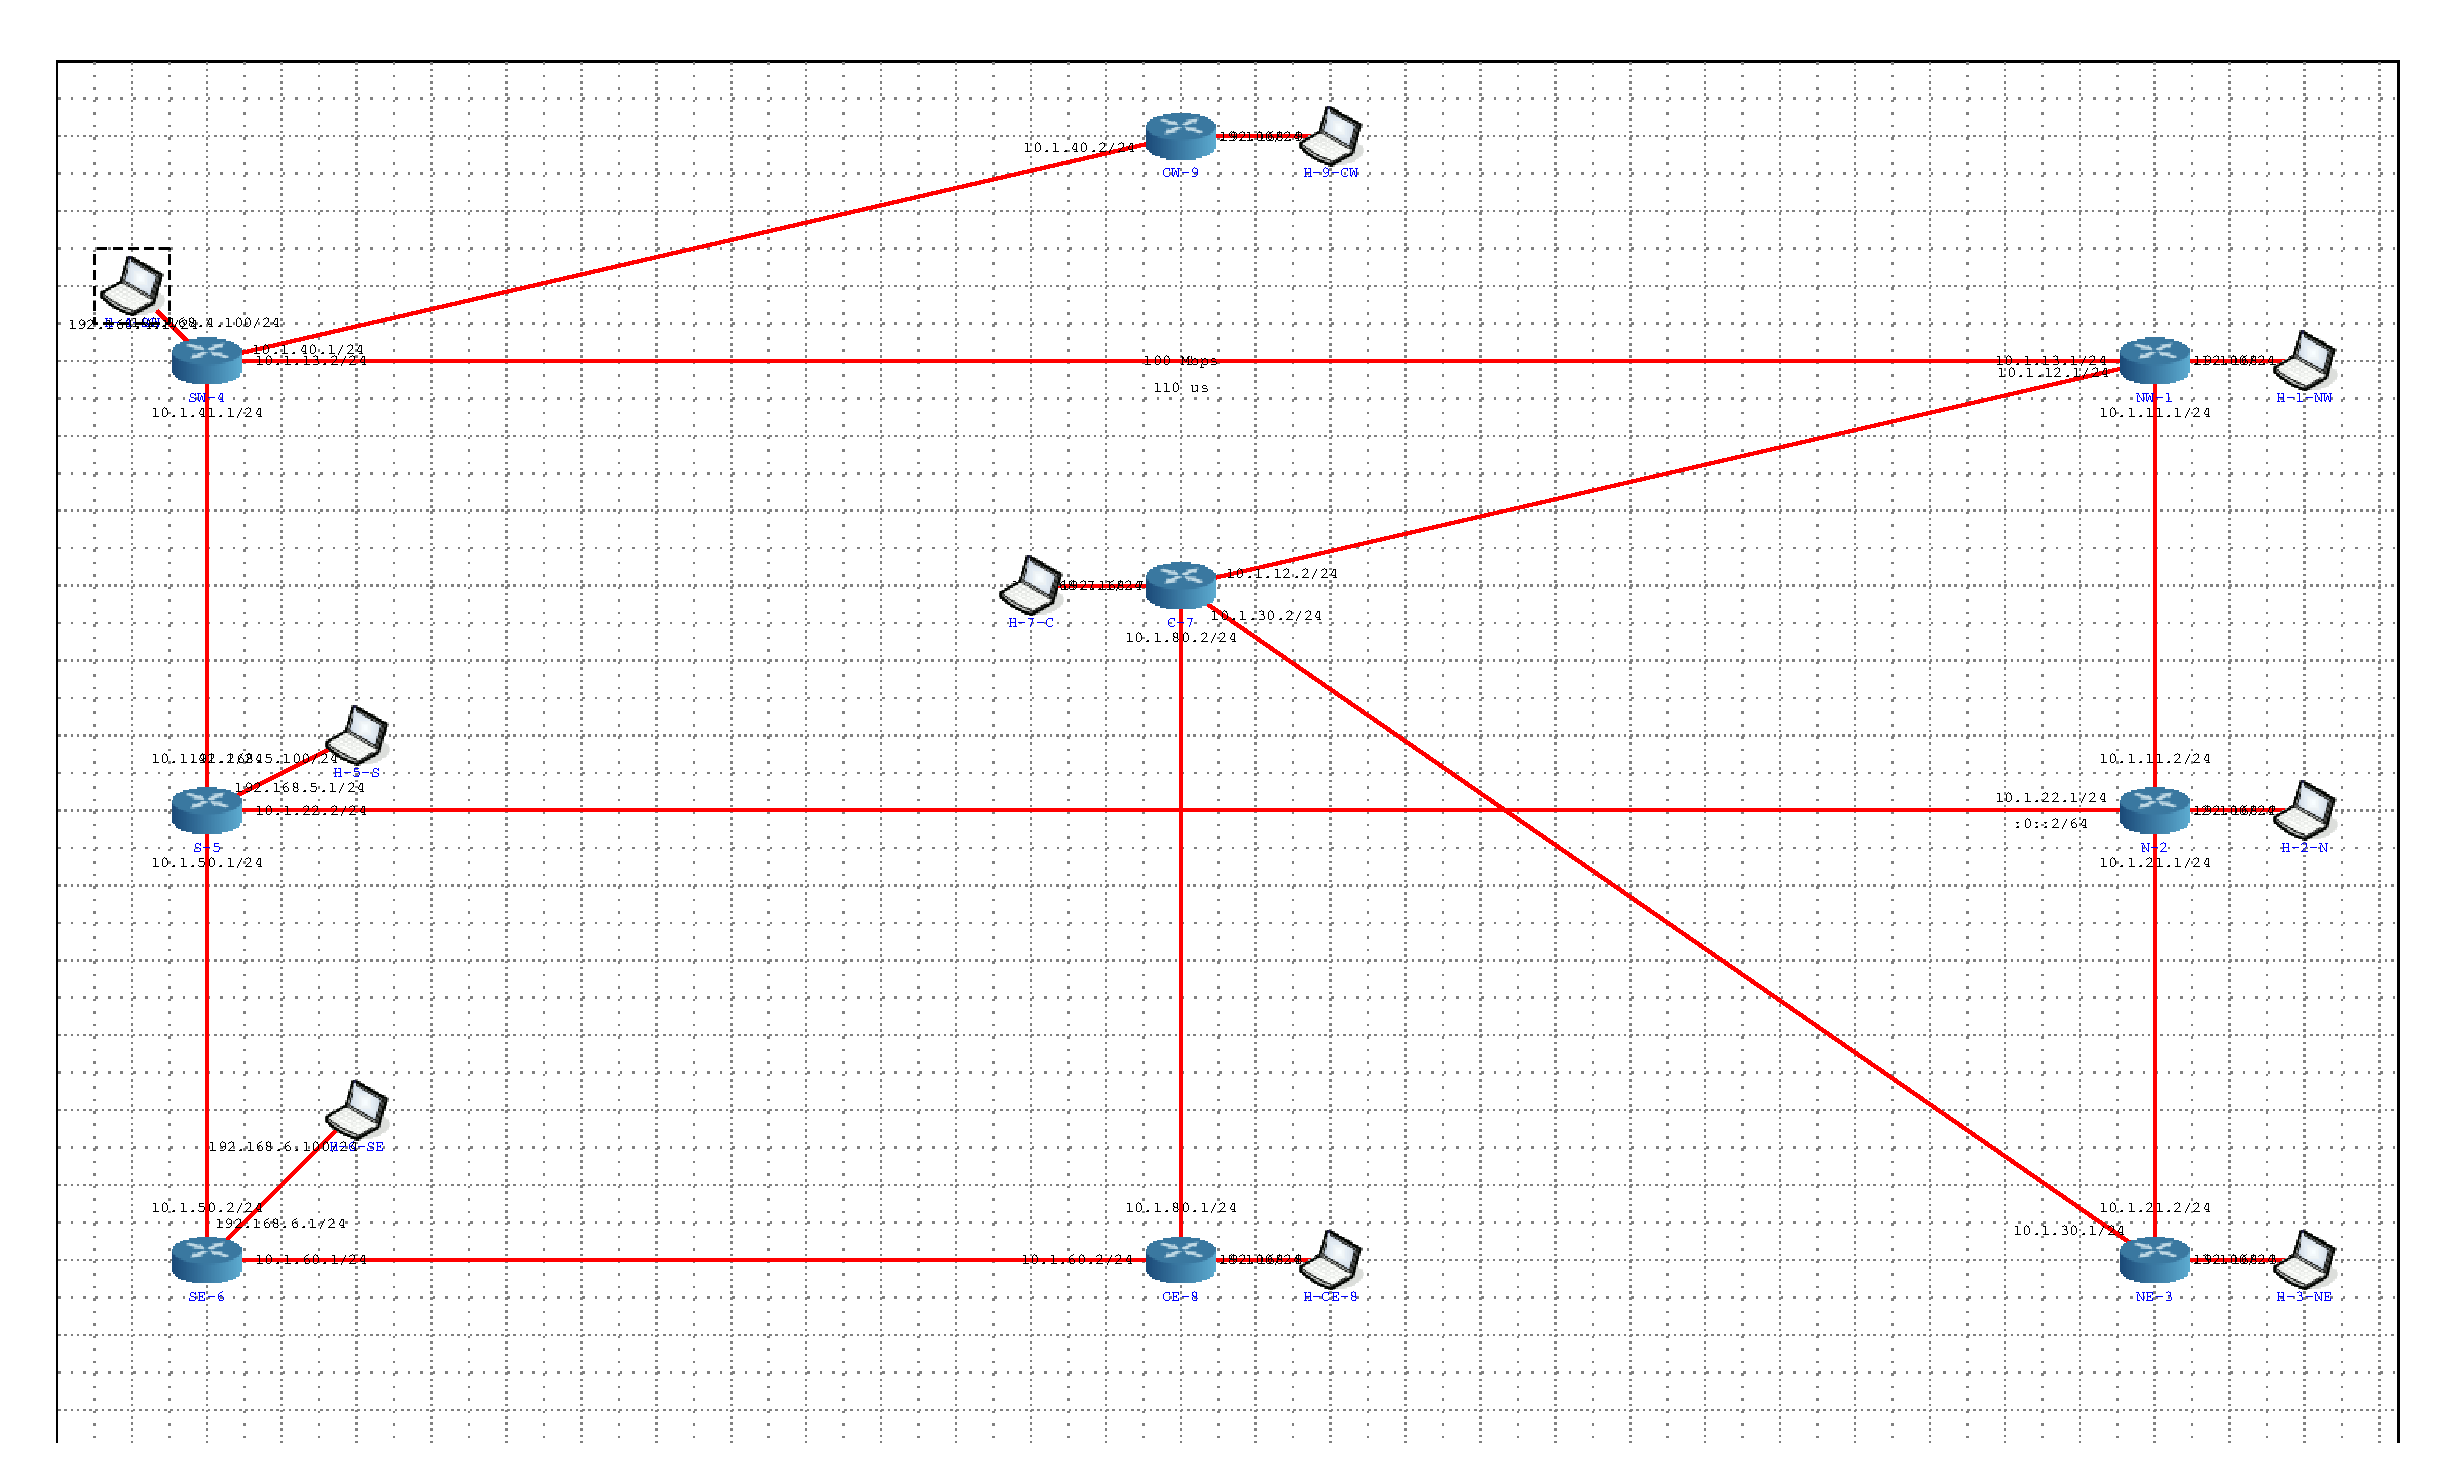
\includegraphics[width=0.8\textwidth]{core-lab3}
  \caption{The ``lab 3 assignment'' as a CORE project}
  \label{fig:core-lab3}
\end{figure}


The Quagga OSPF service can be enabled for the nodes through the graphical interface, and its default configuration will create routes for all the prefixes in all the nodes very quick---no formal measurement was carried out, but after pressing the button and opening a shell on each node, it's immediately possible to ping all other nodes.

We ran a throughput test, with \texttt{iperf3}, between two PCs connected to interconnected routers and the measured speed was $4.49~\mbox{Gbit/s}$, without a memory spike in the containers.

% end of section
